% Mechanism overview figure: generated by paper/mechanism_figure.py, do not edit numbers by hand.
% 1) upload figures/fig_mechanisms.pdf    2) paste the paragraph and the figure environment into main.tex

% --- paragraph
Figure~\ref{fig:mech} collects the mechanisms in one view. The baseline is a rule (Fig.~\ref{fig:mech}a): the strength of a porous sheet is its weakest cross-section times the strength of its ligaments, and the ligament strength depends on the kind of ligament, about 30\,\Nm{} for straight or wide ligaments against 17\,\Nm{} for ligaments narrower than 18\,\AA, in which edge atoms make up a large share of the section (over the 56 meshes the ligament strength correlates with the mean ligament width, $r=0.80$). The two new results of this work are the two ways in which the rule fails. It fails for slit arrays tilted against the load (Fig.~\ref{fig:mech}b), because it counts material and not connectivity: up to $20^\circ$ the overlapping slit tips link en echelon and the strength falls from 25.4 to 8.9\,\Nm; between 25 and $45^\circ$ the ribbons between the slits rotate towards the load and the strength recovers to 18.5\,\Nm; beyond $60^\circ$ every straight load path is cut, the load zigzags through short bridges and the strength falls to 4.0\,\Nm. And it is incomplete for meshes (Fig.~\ref{fig:mech}c), in which the strength at fixed porosity follows the alignment of the solid phase with the load, and a second hierarchical level earns no premium beyond the alignment it provides ($-1.6\pm1.4$\,\Nm{} relative to the one-level trend).

% --- figure
\begin{figure}[!tbp]\centering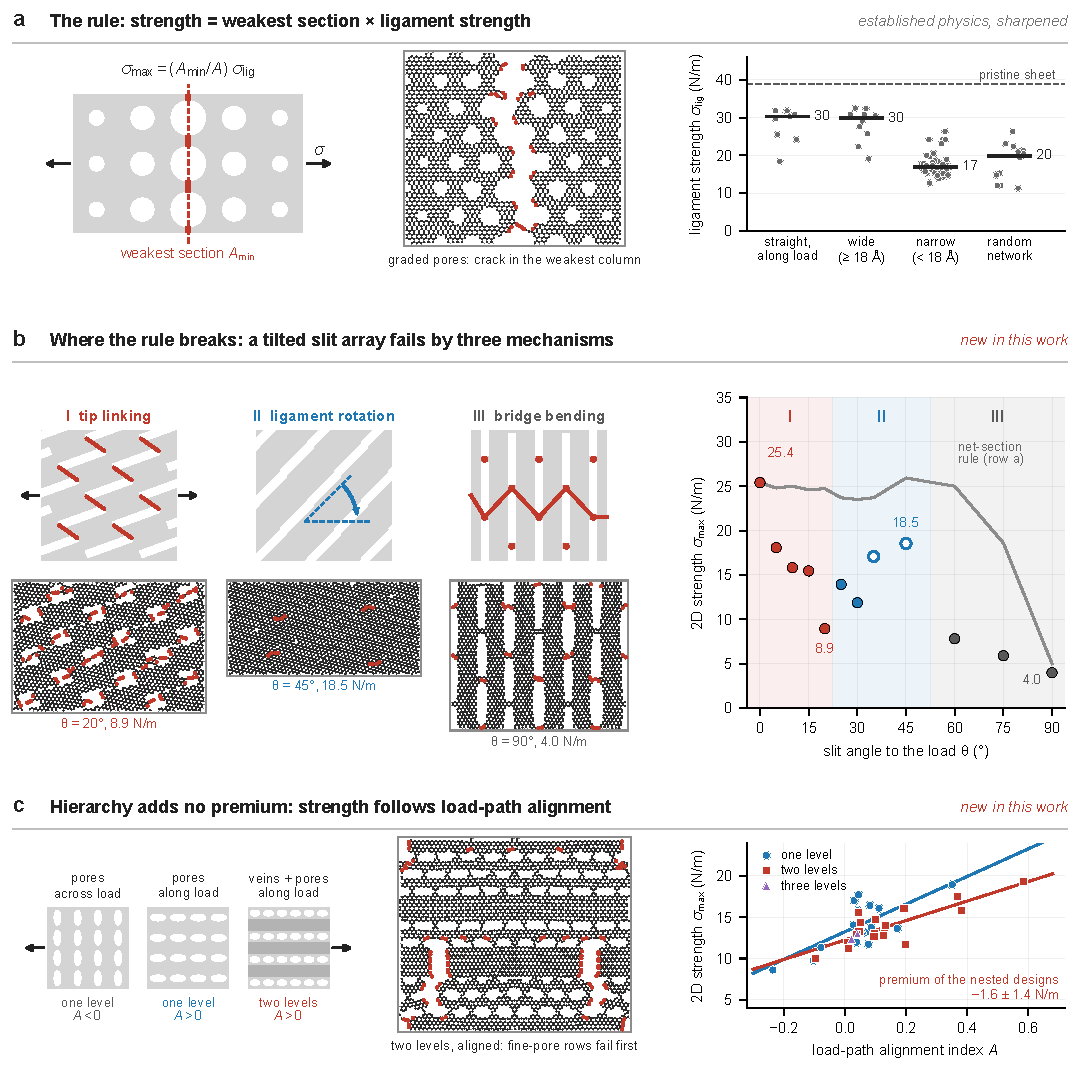
\includegraphics[width=\textwidth]{fig_mechanisms.pdf}
\caption{\textbf{What sets the strength: the rule and the two ways in which it fails.} Each row shows a schematic (left), an atomistic snapshot of the failure (middle; atoms that have lost a bond in red) and one measurement (right). (a) The rule: strength is the smallest solid cross-section perpendicular to the load, $A_\mathrm{min}/A$, times a ligament strength $\sigma_\mathrm{lig}$. In a sheet with graded pores the crack runs through the most porous column. Right: $\sigma_\mathrm{lig}=\sigma_\mathrm{max}/(A_\mathrm{min}/A)$ of the 77 porous designs other than tilted slit arrays, grouped by the ligament classes of the pre-registered predictor (straight along the load; wide, at least 18\,\AA; narrow; random network); bars are medians (30, 30, 17 and 20\,\Nm), the dashed line is the pristine sheet. (b) Where the rule breaks: slit arrays at equal porosity tilted against the load, drawn to scale from the simulated parameters. I, tip linking: the tips of adjacent rows overlap, the slivers between them fail and the cracks link en echelon (red). II, ligament rotation: the ribbons between the slit channels rotate towards the load; at peak load the slits have closed. III, bridge bending: the slits cut every straight load path and the load zigzags through short bridges (red). Right: strength against slit angle for the 12 simulated angles; the net-section rule of row a (grey line) is blind to all three mechanisms; open symbols have porosity 0.18 instead of 0.20. (c) Hierarchy adds no premium: elongating the pores across or along the load changes the load-path alignment index $A$ (Eq.~\ref{eq:A}), and a second level of solid veins along the load is another way of raising $A$. Right: strength against $A$ for the 40 ordered meshes with one, two and three levels and the linear trends for one and two levels; at equal $A$ the nested designs lie $-1.6\pm1.4$\,\Nm{} from the one-level trend. Model results (screened REBO2, athermal quasi-static tension).}
\label{fig:mech}\end{figure}
